\documentclass{article}


\usepackage[round]{natbib}
\usepackage{amsmath,amssymb,amsthm,bm,enumerate,mathrsfs,mathtools}
\usepackage{latexsym,color,verbatim,multirow}
\usepackage{graphicx}
\usepackage{caption}
\usepackage{subcaption}
\usepackage{tikz}
\usepackage{geometry}
\usetikzlibrary{shapes,arrows}
\tikzstyle{block} = [rectangle, draw, fill=white!20,
    text width=7em, text centered, rounded corners, minimum height=4em]
\tikzstyle{title} = [text width=7em, text centered, font=\bfseries]
\tikzstyle{line} = [draw, -latex']


\usepackage{mycommands}

\begin{document}

\newtheorem{theorem}{Theorem}
\newtheorem{corollary}[theorem]{Corollary}
\newtheorem{lemma}[theorem]{Lemma}
\newtheorem{observation}[theorem]{Observation}
\newtheorem{proposition}[theorem]{Proposition}
\newtheorem{definition}[theorem]{Definition}
\newtheorem{claim}[theorem]{Claim}
\newtheorem{fact}[theorem]{Fact}
\newtheorem{assumption}[theorem]{Assumption}
\newtheorem{model}[theorem]{Model}

\theoremstyle{definition}
\newtheorem{example}{Example}

\newcommand{\cM}{\mathcal{M}}
\newcommand{\cH}{\mathcal{H}}
\newcommand{\cD}{\mathcal{D}}
\newcommand{\FDR}{\textnormal{FDR}}
\newcommand{\FCR}{\textnormal{FCR}}
\newcommand{\crt}{\phi}
\newcommand{\M}{\mathcal{M}}
\newcommand{\cY}{\mathcal{Y}}
\newcommand{\cX}{\mathcal{X}}
\newcommand{\cV}{\mathcal{V}}
\newcommand{\bX}{\mathbf{X}}
\newcommand{\x}{\mathbf{x}}
\newcommand{\Gv}{\;\;\big|\;\;}
%\newcommand{\cP}{\mathcal{P}}
\newcommand{\proj}{\cP}
\newcommand{\pow}{\text{Pow}}
\newcommand{\sF}{\mathscr{F}}
\newcommand{\cF}{\mathcal{F}}
\newcommand{\sC}{\mathscr{C}}
\newcommand{\hJ}{\widehat{J}}
\newcommand{\bH}{\mathbf{H}}
\newcommand{\bM}{\mathbf{M}}
\newcommand{\tM}{\widetilde{M}}
\newcommand{\tE}{\widetilde{E}}
\newcommand{\tV}{\widetilde{V}}
\newcommand{\tR}{\widetilde{R}}
\newcommand{\hK}{\widehat{K}}
\newcommand{\hk}{\hat{k}}
\newcommand{\cN}{\mathcal{N}}
\newcommand{\leqAS}{\overset{\textrm{a.s.}}{\leq}}


\newcommand*\mystrut{\vrule width0pt height0pt depth1.5ex\relax}
\newcommand{\underlabel}{\underbracket[1pt][.5pt]{\mystrut \quad\;\; \sub \quad\;\; }}
\newcommand{\JTcomment}[1]{{\color{blue}{(JT: \bf \sc #1) }}}
\newcommand{\WFcomment}[1]{{\color{red}{(WF: \bf \sc #1) }}}

\title{Adaptive Sequential Model Selection}
\author{William Fithian, Jonathan Taylor, Rob Tibshirani, and Ryan Tibshirani}
\maketitle

\begin{abstract}
  Many model selection algorithms produce a ``path'' of fits that can be veiwed as specifying a sequence of models of increasing complexity. Given such a sequence of models and the data set used to produce them, we consider the problem of choosing the least complex model that is not falsified by the data, while accounting for the fact that the model path is determined adaptively using the data. Extending the tools of Fithian, Sun and Taylor (2014), we construct a $p$-value for each step in the sequence. In the case of linear regression, our $p$-values improve on the power of the spacings test of \citet{taylor2014exact}, often dramatically. By combining our $p$-values with stopping rules proposed by \citet{gsell2013sequential}, we achieve adaptive control of the pathwise familywise error rate and false discovery rate.
\end{abstract}


\section{Introduction}

... generates a sequence of increasingly complex models. Our goal is to choose the simplest model that is not falsified by the available data.

... and find the index of the smallest adequate model --- that is, the smallest model that cannot be falsified given available evidence.

\begin{example}[Forward-Stepwise Linear Regression with the LASSO]
  \citet{taylor2014exact}
\end{example}

\begin{example}[The LARS Algorithm in Regression]
  \citet{taylor2014exact}
\end{example}

\begin{example}[Ever-Active Path in $\ell_1$-Regularized Methods]
  \citet{taylor2014exact}
\end{example}

\begin{example}[Principal Components Analysis]
  As a second motivating example, consider model selection for   principal components analysis. In that case we are given a data matrix $X \in \R^{n\times d}$, with which we form a sample covariance matrix
\[
S = \frac{1}{n-1} \sum_{i=1}^n(x_i - \bar x)^2
\]
The first $d$ principal component loadings are the first $d$ eigenvectors of $S$, which call $u_1,\ldots, u_d$. These induce a sequence of nested Wishart models:
\[
M_0 \sub M_1 \sub \cdots \sub M_d
\]
in which
\begin{equation}
  M_k:\; (n-1) S \sim W_d\left(\lambda_0 I_d + \sum_{\ell=1}^k     \lambda_\ell u_i u_i', \;\;\; n-1\right).
\end{equation}
This problem was studied in \citet{choi2014selecting}.
\end{example}

\subsection{Generic Setting}

More generically, we observe data $Y \in \cY$, with unknown sampling distribution $F$. We then use $Y$ to generate an adaptive sequence of $d$ nested models
\[
M_0(Y) \sub M_1(Y) \sub \cdots \sub M_d(Y).
\]
Define the {\em completion index} $k_0(Y) = \min\{k:\; F \in M_k\}$, the index of the first correct model. 

We will consider two related problems. First, we will consider the problem of obtaining selective single-step $p$-values, where $p_k$ is a $p$-value for testing
\[
H_{0,k}:\; F\in M_{k-1}\quad \text{ vs. } \quad 
H_{1,k}:\; F\in M_k\setminus M_{k-1},
\]
while adjusting for the fact that the models are chosen adaptively. As we will see, {\em selected-model} tests can be dramatically more powerful than {\em saturated-model} tests at early steps in the model path when most of the signal variables have not yet entered the model.

The second half of the paper concerns {\em stopping rules} $\hk$, estimators of $k_0$. We will consider several stopping rules that operate on the full sequence $p_{[d]}$, including two powerful stopping rules proposed in \citet{gsell2013sequential}. These latter require guarantees on the joint law of the $p$-values. We will prove sufficient conditions for when the $p$-values are Gaussian.

Although we will focus most of our attention and examples on the case of selecting a set of predictors in linear regression, essentially all of our results apply in generic exponential family models.

\subsection{Which Null Hypothesis Should We Test?}

There is some ambiguity involved in deciding how to generalize $z$- and $t$-tests to the selective case. For example, \citet{gsell2013sequential} describe three different null hypotheses that we could consider testing at step $k$. As discussed at some length in \citet{fithian2014optimal}, there are several different models that 

In some cases the design matrix of the full model may represent a  scrupulously curated set of features, and the analysts may know in advance that inferences with respect to the full model are of major scientific interest. For example, the scientist may believe, due to theoretical considerations, that a nonzero coefficient of $X_1$ after controlling for $X_2,\ldots,X_p$ would be evidence for a causal effect of $X_1$ on the response.

If the full model has no special scientific status, however, then we see little advantage in insisting that all inferences should adjust for every other predictor in the full design matrix $X$. For example, suppose that $X$ contains gene expression measurements for all genes that happened to be measured by a microarry chip. Then $\beta_{j,\text{Full}}$ is already fairly arbitrary, since we would be controlling for a different set of genes if we had purchased the chip from a different manufacturer.

\WFcomment{Also say: Controlling for more variables could take us farther from a causal effect; furthermore, coefficient in larger model is much harder to interpret.}


\section{Inference for One Step}

To begin, we consider the problem of constructing a valid selective $p$-value for a particular step. At step $k$, we construct $p_k(Y)$ to test
\[
  H_{0,k}:\; F \in M_{k-1}(Y)
  \quad \text{ vs. } \quad
  H_{1,k}:\; F \in M_k(Y) \setminus M_{k-1}(Y).
\]
The main complication arises from the fact that the null and alternative hypotheses are random. To simplify matters, we first consider deriving $p$-values for a fixed candidate pair $m_{k-1} \sub m_k$.

The random variable  $p_{k,m_{k-1},m_k}(Y)$ is a valid {\em selective $p$-value} for the fixed candidate pair $(m_{k-1},m_k)$ if it is stochastically larger than uniform under the (fixed) null $m_{k-1}$, given that the pair $(m_{k-1},m_k)$ is selected. That is,
\[
\P_F\left(p_{k,m_{k-1},m_k}(Y) \leq \alpha \mid M_{k-1}(Y) = m_{k-1}\right) 
\leq \alpha, \quad \forall F\in m_{k-1}, \alpha \in [0,1].
\]
Given selective $p$-values for each fixed candidate pair, we can construct a combined $p$-value for the random null $(M_{k-1},M_k)$: 
\[
p_k(y) = p_{k, M_{k-1}(y), M_k(y)}(y),
\]
which is a valid $p$-value on the event $\{F \in M_{k-1}(Y)\}$:
\[
\P_F\left(p_k \leq \alpha \mid M_{k-1}, \;M_k, 
  \;F\in M_{k-1}\right) \leq \alpha, \quad \forall \alpha \in [0,1].
\]
Recall that, as usual, $F$ is not random, but $M_{k-1}$ is.

Methods for one-step selective $p$-values are by now well-studied. \WFcomment{big list of references.} See \citet{fithian2014optimal} for a general treatment. 

\subsection{Selective $p$-Values in Regression}

\subsection{Selected- and Saturated-Model inference}

We illustrate the superior power of the selected-model test in early steps with an extended example.

\begin{example}[Bivariate Regression]\label{ex:bivariate}
  Consider forward stepwise selection in a regression model with $n=p=2$, with identity design $X = I_2=\begin{pmatrix} 1 & 0 \\ 0 & 1\end{pmatrix}$ and known $\sigma^2=1$. We perform one step of forward stepwise and then test the null model with no variables against the model with one variable. 

We will choose variable 1 first on the selection event $A=\{|Y_1| > |Y_2|\}$, which is shown in yellow in Figure~\ref{fig:bv_condSets}. In that case,
\[
M_0:\; Y\sim \cN(0,I_2), \quad\text{ and } 
M_1:\; Y \sim \cN\left(\frac{\mu_1}{0}, \; I_2\right).
\]
The selected-model test compares $Y_1$ to its distribution under $M_0$ conditional on $A$, a test of $H_0:\;\mu_1=0$ in model $M_1$.

By contrast, the saturated-model test is a test of $H_0:\; \mu_1=0$ in the model $M_{\text{sat}}:\; Y \sim \cN(\mu, I_2)$. Now, $\mu_2$ enters the problem as a nuisance parameter because the saturated-model test refuses to assume that $\mu_2=0$. To eliminate the nuisance parameter $\mu_2$, the saturated model test must condition on $Y_2$, and compare $Y_1$ to its null distribution given $A$ {\em and} the observed value of $Y_2$.

Figure~\ref{fig:bv_condSets} shows the conditioning sets for each model when $Y=(2.9,2.5)$. Next to it, Figure~\ref{fig:bv_nullDists} shows the null distribution for the test statistic $Y_1$ in each case. The $p$-values for the selected and saturated models are 0.007 and 0.3, respectively. These two plots are reproduced from \citet{fithian2014optimal}, in which the same example was presented in less detail.
\end{example}

\begin{figure}
  \centering
  \begin{subfigure}[t]{.4\textwidth}
    % source code: bivariateSelVSat.R
    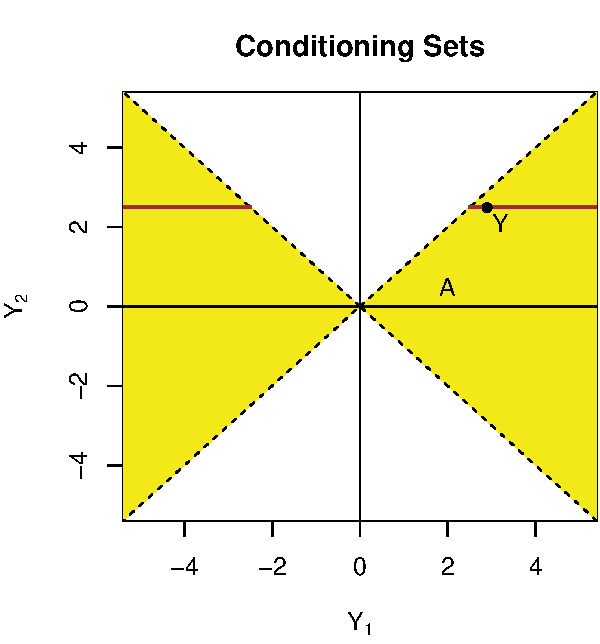
\includegraphics[width=\textwidth]{figs/bivariateSelVSat_condSets.pdf}
    \caption{\WFcomment{Copied directly from FST14; reword} 
      For $Y=(2.9,2.5)$, the selected-model conditioning set is
      $A=\{y:\;|y_1|>|y_2|\}$, a union of quadrants,
      plotted in yellow. The saturated-model conditioning set
      is ${\{y:\; y_2=2.5\}\cap A} = {\{y:\;y_2=2.5, |y_1|>2.5\}}$,
      a union of rays, plotted in brown.}
    \label{fig:bv_condSets}
  \end{subfigure}
  \hspace{.1\textwidth}
  \begin{subfigure}[t]{.4\textwidth}
    % source code: bivariateSelVSat.R
    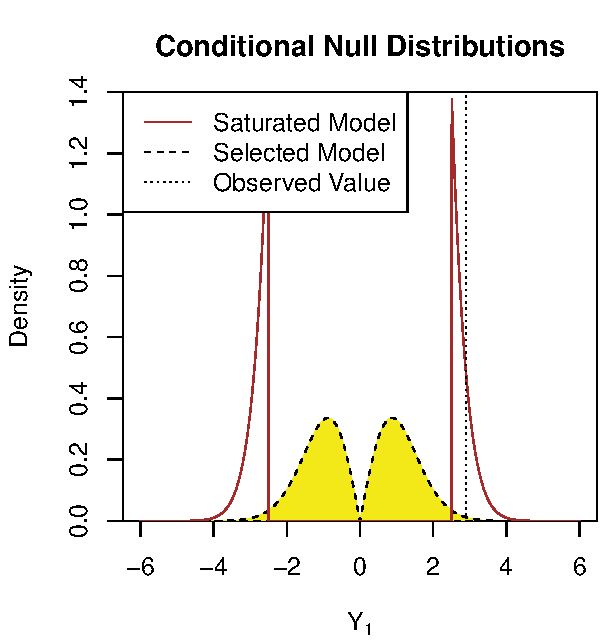
\includegraphics[width=\textwidth]{figs/bivariateSelVSat_nullDists.pdf}
    \caption{\WFcomment{Copied directly from FST14; reword} 
      Conditional distributions of $Y_1$ under
      $H_0:\mu_1 = 0$. Under the hypothesis
      $\mu=0$, the realized  $|Y_1|$ is  quite large given $A$,
      giving  $p$-value 0.015. By contrast, $|Y_1|$ is not too large
      given $A \cap \{y:\; y_2=Y_2\}$, giving
      $p$-value 0.3.}
  \end{subfigure}
  \caption{\WFcomment{Copied directly from FST14; reword} 
    Contrast between the saturated-model and selected-model tests
    in Example~\ref{ex:bivariate}, in which we fit a one-sparse model with
    design matrix $\bX=I_2$. The selected-model test is based
    on  $\L_0(Y_1 \gv A)$, whereas the saturated-model test is based
    on $\L_0(Y_1  \gv  Y_2, A)$.}
  \label{fig:bv_nullDists}
\end{figure}


The case illustrated in Figure~\ref{fig:bv_condSets} exhibits a phenomenon that has been remarked upon elsewhere in the literature of saturated-model tests: when there are near-ties between strong variables that are competing to enter the model, the winning variable may have a very weak $p$-value. \WFcomment{add references}. Figure~\ref{fig:bv_rocCurve} displays the cumulative distribution function for the first $p$-value when $\mu=\binom{4}{4}$, a very strong signal. While the selected model test has near perfect power, it is not uncommon for the saturated model test to produce large $p$-values, even in the range of 0.5-0.9. These large $p$-values arise exactly when there is a near tie between the variables.

\begin{figure}
  \centering
  % source code: bivariateSelVSat.R
  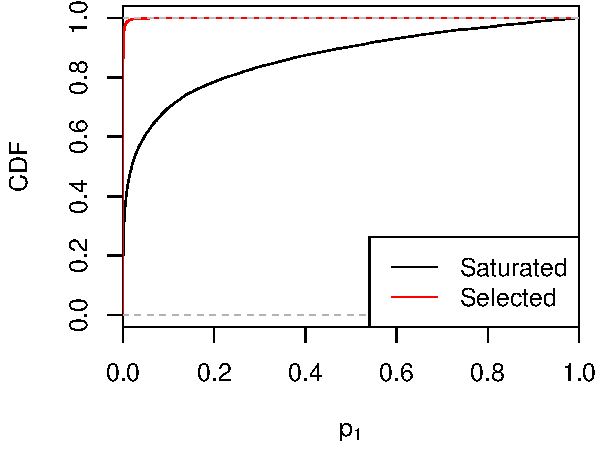
\includegraphics[width=.5\textwidth]{figs/bivariateSelVSat_rocCurve.pdf}
  \caption{\WFcomment{Write caption here.}}
  \label{fig:bv_rocCurve}
\end{figure}

Results in \citet{fithian2014optimal} show that the selected-model test is strictly more powerful when the selected model is correct; i.e., when $\mu_2=0$. Figure~\ref{fig:bv_powCurves_0} shows the power curve for each test when $\mu_2=0$. While the selected-model test is more powerful, the difference between the two is relatively mild. Interestingly, the difference is much more pronounced when $\mu_2=4$, as shown in Figure~\ref{fig:bv_powCurves_4}.

\begin{figure}
  \centering
  \begin{subfigure}[t]{.4\textwidth}
    % source code: bivariateSelVSat.R
    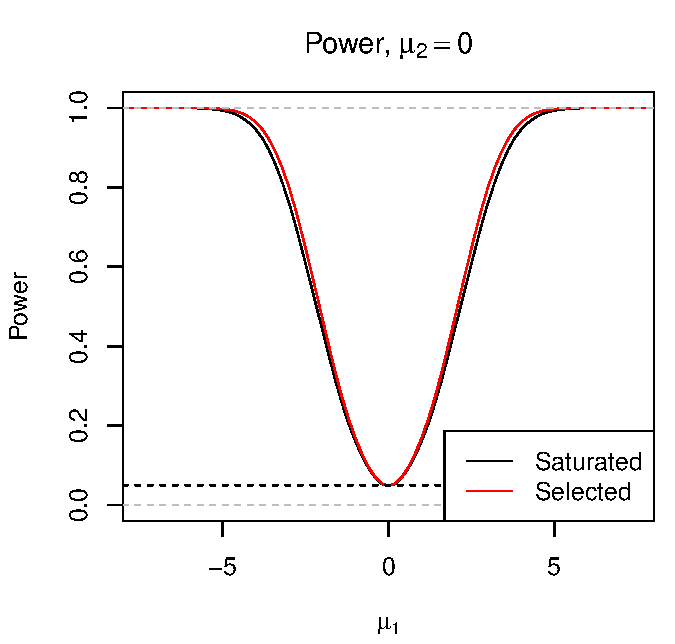
\includegraphics[width=\textwidth]{figs/bivariateSelVSat_powCurves_0.pdf}
    \caption{\WFcomment{Write caption here.}}
    \label{fig:bv_powCurves_0}
  \end{subfigure}
  \hspace{.1\textwidth}
  \begin{subfigure}[t]{.4\textwidth}
    % source code: bivariateSelVSat.R
    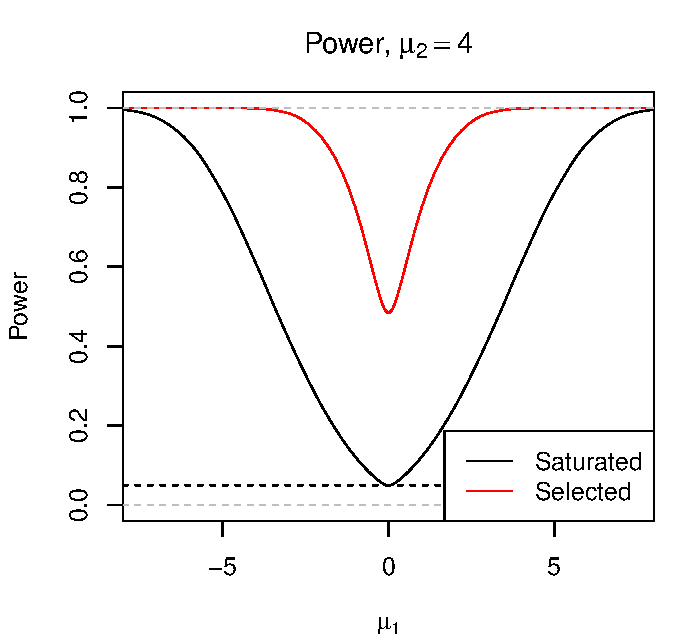
\includegraphics[width=\textwidth]{figs/bivariateSelVSat_powCurves_4.pdf}
    \caption{\WFcomment{Write caption here.}}
  \end{subfigure}
  \caption{\WFcomment{Write caption here.}}
   \label{fig:bv_powCurves_4}
\end{figure}



\section{Sequential Inference}

Having discussed methods for constructing single-step $p$-values, we turn now to the problem of constructing a {\em stopping rule}; that is, an estimator $\hk$ of the completion index $k_0(Y)\in \{0,\ldots,d,\infty\}$. $M_k$ is ``rejected'' if and only if $\hk>k$. Thus $\hk$ is the number of models we rejected, while $k_0$ is the number that we should have rejected. The number of type I errors, then, is $(\hk-k_0)_+$, while the number of type II errors is $(k_0-\hk)_+$. Define $V=(\hk-k_0)_+$, the number of excess rejections.

Note that the type I error $V$ is defined in a ``model-centric,'' as opposed to a ``variable-centric,'' fashion: in regression, our model-wise $V$ counts the number of true null {\em models} incorrectly rejected, instead of counting the number of noise variables included in the final model. We can define the (model-wise) familywise error rate (FWER) and false discovery rate (FDR) respectively as $\P_F(V >0)$ and $\E_F[V/(\hk \vee 1)]$. 

We could have instead defined the ``variable-centric'' type I error $\tV$ as the number of noise variables incorrectly included in the final model, with $\tR$ denoting the total number of variables included. Here, by ``noise variable'' we mean one that has a non-zero coefficient in the full model. Using selective inference to control the variable-wise FWER $\P_\mu(\tV>0)$ and FDR $\E[\tV / (\tR \vee 1)]$ is an interesting topic for further study.

\subsection{Stopping Rules}

We will consider stopping rules that depend on the sequence $p_1,\ldots,p_d$ of $p$-values, which have been studied in the literature by \WFcomment{literature review here.} We will focus on three such stopping rules: simple stop, proposed by \WFcomment{whom?}, and the more refined strong stop and forward stop, proposed by \citet{gsell2013sequential}. 

While strong stop and forward stop tend to give more powerful stopping rules, they require independence among the $p$-values. Sections~\ref{sec:modelSPSP}--\ref{sec:pvalSP} discuss conditions on the model sequence $M_{[d]}$ and the $p$-value sequence $p_{[d]}$ under which selective $p$-values are mutually independent. We will see that, typically, selected-model $p$-values are sequentially independent while saturated-model $p$-values are not.

\subsubsection{Basic Stop:}

\WFcomment{Is there a better name for this? Can we find it in the literature?}

The most obvious sequential procedure is to reject at each step until the first time $p_k > \alpha$, which we can formalize as
\[
\hk_B(Y) = \min\left\{k \in \{1,\ldots,m\} :\;
  p_k > \alpha\right\} - 1
\]
We will call this procedure ``basic stop.'' 

If $k_0$ is fixed, then it is clear that $\hk_b$ controls the FWER at level $\alpha$ provided that $p_{k}$ is a valid $p$-value for each $k>k_0$. Then, 
\[
\P(V>0) = \P(p_{k_0+1} \leq \alpha) \leq \alpha
\]
\WFcomment{Trivial, but no doubt someone else proved this first...}

Selectively valid single-step $p$-values do not necessarily guarantee FWER control when $k_0$ is random. In that case, we need a bit more, but it is sufficient that we have type I error control for $p_k$ conditional on $k_0=k-1$; i.e., not just conditional on $M_{k-1}$ being a correct model, but given that $M_{k-1}$ is the {\em first} correct model.

\subsubsection{Strong Stop:}

\citet{gsell2013sequential} propose another method for controlling the model-wise FWER, which they called ``strong stop.'' Define
\[
  \hk_{S}(Y) = \max\left\{k \in \{1,\ldots,d\} :\;
    \exp\left(\sum_{i=k}^d \frac{\log p_i}{i}\right) 
    \leq \frac{\alpha k}{d}\right\}
\]
Even if $p_k$ is a little larger than $\alpha$, say $\alpha=0.05$ and $p_k=0.06$, strong stop can still reject $M_{k-1}$ if the next three or four $p$-values are also relatively small.

\citet{gsell2013sequential} show that if $k_0$ is fixed, then $\hk_S$ controls the FWER at level $\alpha$, as long as the null $p$-values are independent given the non-null ones. Specifically, they require that
\[
\P(p_{k_0+1} \leq \alpha_{k_0+1}, \ldots, p_d \leq \alpha_d
\mid p_1, \ldots, p_{k_0}) \leq \prod_{\ell=k_0+1}^d \alpha_\ell
\]


\subsubsection{Forward Stop:}


\subsection{Independent $p$-Values and Sufficiency Principles}


\subsection{}

\subsubsection{A Sub-Path Sufficiency Principle for SelectionAlgorithms}\label{sec:modelSPSP}


\subsubsection{A Sub-Path Sufficiency Principle for SelectionAlgorithms}\label{sec:modelSPSP}

We say that a selection algorithm $M_{[d]}(\cdot)$ satisfies the {\em sub-path sufficiency principle} (henceforth SPSP) if, given $M_k(Y)=m_k$, the sequence of models $M_{[k]}$ depends only on sufficient statistics of $m_k$. That is


A model selection procedure derived from the ``ever-active'' coefficients of a regularized likelihood path always satisfies the SPSP. Let $M_\infty$ be a model with parameters $\theta\in\Theta\sub \R^p$, and likelihood $L(\theta; Y)$. For $r=0,\ldots,R$, let $P_r(\theta)$ denote a sequence of regularizing penalties, and define
\begin{align}\label{eq:regPathDef_start}
  \hat\theta^{r}(Y) &\triangleq 
  \argmin_{\theta\in\Theta} -\log L(\theta; Y) + P_r(\theta) \\
  \tE_r(Y) &\triangleq \left\{j:\; \hat\theta_j^s \neq 0 
    \text{ for any } s \leq r \right\}
\end{align}
Note that while the sets $\tE_r$ are nested by definition, we could have $\tE_r = \tE_{r+1}$ for most values of $r$. Let $r(0)=0$, and for $k>0$ define
\begin{equation}
r(k) = \min\{s:\; \tE_s \neq \tE_{r(k-1)}\}.
\end{equation}
That is, the $r(k)$ are the indices where the active set changes. Let $E_k = \tE_{r(k)}$, and take
\begin{equation}\label{eq:regPathDef_end}
M_k \triangleq \{F\in M_\infty:\; \theta_j = 0,\; \forall j \notin E_k\}
\end{equation}
Model paths described in this way satisfy the SPSP, as we see next.

\begin{proposition}[Regularized Likelihood Paths Satisfy SPSP]
  Model paths specified as in (\ref{eq:regPathDef_start}--\ref{eq:regPathDef_end}) satisfy the sub-path sufficiency principle.
\end{proposition}
\WFcomment{Actually, you just keep the times when the model changes... Need to recast notation a bit; indices of $\lambda$ (or $P$, here) need not match up with indices of model.}

\begin{proof}
  Let 
\end{proof}

\begin{proposition}[Forward Stepwise Paths Satisfy SPSP]
  \WFcomment{Generalized forward stepwise}
\end{proposition}

\begin{proof}
  Let
\end{proof}

\WFcomment{There is a filtration interpretation when you have the appropriate sufficiency properties.} Let $\sF_{k,\ell}$ denote the $\sigma$-algebra generated by $M_{[k]}$ and $p_{[\ell]}$.
\begin{align*}
  \sF_{k,\ell} &= \sF(M_{[k]},p_{[\ell]})\\
  \sF_0 &\underlabel_{\text{selection } 1} \sF_{1,0} \underlabel_{\text{inference } 1}
  \sF_{1,1} \;\;\sub \cdots \sub\;\;
  \sF_{d-1,d-1} \underlabel_{\text{selection } d} \sF_{d,d-1}
  \underlabel_{\text{inference } d} \sF_{d,d}
\end{align*}

\subsection{}



\section{Simulation: Sparse Linear Regression}


\section{Simulation: Principal Components Analysis}

\WFcomment{Can we do this one?}

\bibliographystyle{plainnat}
\bibliography{biblio}

\end{document}
